\documentclass{article}
\usepackage[preprint]{neurips_2026}
\usepackage[utf8]{inputenc}
\usepackage[T1]{fontenc}
\usepackage{graphicx}
\usepackage{booktabs}
\usepackage{amssymb}
\usepackage{amsmath}
\usepackage{hyperref}
\usepackage{caption}
\usepackage{tikz}
\usetikzlibrary{positioning,arrows.meta}

\title{When More Reward Signal Does Not Help: A Controlled Study of Reward Decomposition for GRPO Debugging}
\author{Shashaank Jain \and Pranav Pulipati}

\begin{document}

\maketitle

\begin{center}
\textit{Code, dataset, per-bug results, and pre-registration: \url{https://github.com/shasshaank/AgentDebuggerEnv}}
\end{center}

\vspace{0.3cm}
\noindent \textbf{Keywords:} reinforcement learning, reward shaping, GRPO, program repair, verifiable rewards, generalization, negative results, evaluation methodology
\vspace{0.3cm}

\begin{abstract}
Hand-crafted reward decompositions are often used in reinforcement learning for language models to provide intermediate learning signals before a policy reliably achieves verifiable outcomes. We test whether such reasoning-targeted shaping improves GRPO training for program debugging. We train Qwen2.5-Coder-3B-Instruct with GRPO and LoRA on 90 single-function Python bugs under three pre-registered reward configurations: a seven-component dense reward (R0), a graded executable outcome reward with regression penalties (R1), and a dense reward with the two reasoning-targeted components removed (R2). All three RL configurations share the same model, data, prompts, optimizer, curriculum, and evaluation procedure. On 90 held-out bugs, R0 achieves a 45.6\% solve rate, compared with 48.5\% for R1 and 48.5\% for R2. Paired bootstrap analysis gives a 95\% interval of [$-$8.5, $+$2.6] percentage points for R0$-$R1, ruling out an advantage for the dense reward larger than 2.6 percentage points at the reported confidence level. The nine RL runs achieve a pooled mean held-out solve rate of 47.5\%, which is 9.7 percentage points above the structured zero-shot baseline (37.8\%), but only 1.9 percentage points above the unconstrained free-form zero-shot baseline (45.6\%). This pattern is consistent with GRPO primarily recovering performance lost to the structured-response constraint rather than producing a large increase in underlying repair capability. Crucially, under group size $G=2$, sample standard deviation normalization eliminates the magnitude of reward differences, scaling any non-zero reward delta to the same absolute advantage magnitude ($\pm 1/\sqrt{2}$, ignoring the numerical stabilizer). Consequently, the 45.7 percentage point reduction in degenerate groups observed under R0 reflects equal-magnitude normalized advantages driven by converting some otherwise degenerate test-outcome groups into heuristic tie-breakers, rather than finer optimization toward functional correctness. An exploratory evaluation on 27 adapted QuixBugs programs yields solve rates between 39.5\% and 44.4\%, serving as a descriptive sanity check against policy collapse on out-of-distribution code, though the absence of an untrained baseline precludes claims of positive transfer. In this controlled single-turn program-repair setting using Qwen2.5-Coder-3B-Instruct and GRPO with $G=2$, the tested seven-component dense reward substantially reduces measured reward degeneracy but does not improve held-out repair accuracy over the simpler graded outcome reward, while the $G=2$ mathematical analysis provides a mechanistic explanation for how such shaping converts outcome ties into same-magnitude heuristic advantages.
\end{abstract}

\section{Introduction}
Reinforcement learning from verifiable rewards has become an increasingly common approach to improving language-model performance on tasks with checkable outcomes, including mathematics and code \cite{Shao2024, Guo2025}. A recurring design question in these systems is how much reward decomposition is useful beyond executable outcomes. Although test execution provides a verifiable signal, sampled fixes can produce similar test outcomes within a GRPO group, leaving little relative reward variation. A natural response is to decompose the reward into hand-crafted components that pay for intermediate desiderata: emitting the required format, stating a specific hypothesis about the fault, naming the buggy function, or resembling the reference solution. The implicit claim is that these additional signals provide useful within-group resolution before the policy reliably produces passing fixes.

The question is not whether dense rewards can increase the numerical reward assigned to intermediate behavior. They obviously can. The question is whether these additional signals improve the policy's eventual ability to produce test-passing fixes when the executable outcome remains available. We therefore hold the model, prompts, data, optimizer, curriculum, and evaluation fixed and vary only the reward decomposition. 

Two structural characteristics of our setting govern how reward signals propagate. First, our setting is single-turn (the model produces the entire proposed fix in one completion), so intermediate reasoning is not an environment transition; dense components shape the scalar reward assigned to a complete response rather than providing temporal credit assignment across steps. Second, under group size $G=2$, GRPO sample standard deviation normalization scales every non-zero reward difference to the same absolute advantage magnitude ($\pm 1/\sqrt{2}$, ignoring the numerical stabilizer). Reward magnitude is eliminated: any reward difference, however minor, yields the same advantage weight. Dense shaping in this regime does not provide finer advantage scaling—it acts strictly as a tie-breaker whenever it alters the relative ordering of two completions.

We test this claim directly in a setting small enough to control completely. We built a debugging environment in which every candidate fix executes in a hardened sandbox against the bug's test cases, and a seven-component dense reward (R0) is implemented as a set of component ceilings on a single scoring class. An ablation is therefore a configuration, not a fork: R1 zeroes every shaping component and rescales the test-outcome term to the same range; R2 zeroes exactly the two reasoning-targeted components and keeps the rest. The three configurations were pre-registered, together with the hypotheses, statistical tests, and threats to validity, before any experiment ran.

On 90 held-out bugs, we find no statistically detectable difference between the reward configurations. The point estimate for graded outcome reward matches or slightly exceeds the full dense reward (48.5\% vs 45.6\%), and the paired bootstrap 95\% confidence interval ([-8.5, +2.6] pp) rules out a dense-reward advantage larger than 2.6 percentage points conditional on the observed training seeds. Furthermore, while RL achieves a 9.7 percentage point gain over the structured zero-shot baseline (37.8\%), the unconstrained free-form zero-shot baseline reaches 45.6\% on the exact same held-out split. The actual gain of RL over the base model's unconstrained capability is only +1.9 pp (small relative to the across-seed variation observed among the RL arms), consistent with the policy primarily recovering performance lost to the structured-format constraint.

Our contributions are:
\begin{itemize}
\item A controlled three-arm experiment isolating the effect of reasoning-targeted reward decomposition in GRPO program repair.
\item An analysis showing that at $G=2$, sample standard deviation normalization eliminates reward magnitude, so dense shaping reduces degenerate GRPO groups (from 61.9\% to 16.2\%) by converting some otherwise degenerate test-outcome groups into equal-magnitude heuristic tie-breaker advantages, which fails to improve held-out repair.
\item An empirical demonstration that RL's apparent +9.7 pp gain over structured zero-shot is consistent with recovering format-induced performance loss rather than general repair improvement over the unrestricted free-form baseline (45.6\%).
\item A methodological case study on generation budget sensitivity and prompt-format penalties in code-RL evaluation.
\end{itemize}

\section{Related Work}

\subsection{Reward Shaping}
Classical potential-based reward shaping provides conditions under which shaping preserves optimal policies \cite{Ng1999}. Our response-level heuristics do not satisfy those conditions, so they could in principle change the learned policy. The experiment asks whether those additional signals improve optimization in practice.

Process-supervision studies give conflicting guidance: process-based feedback can improve the faithfulness of reasoning traces \cite{Lightman2023}, yet outcome-only supervision often matches it on final-answer accuracy \cite{Uesato2022}. Our result provides a small-scale controlled data point consistent with the practical appeal of simple rule-based outcome rewards, as recently highlighted by large-scale RL systems that deliberately avoid learned process rewards \cite{Guo2025}.

\subsection{Code Repair and Evaluation}
Automated program repair using LLMs is a highly active area. Benchmarks like MBPP and QuixBugs \cite{Lin2017} are heavily utilized to evaluate code generation and debugging. Recent work has increasingly stressed the importance of robust evaluation frameworks, as subtle prompt or parsing artifacts can artificially suppress or inflate model scores \cite{Tian2024, Tam2024}.

\subsection{Spurious Rewards and Elicitation in RLVR}
Recent studies have challenged the assumption that reinforcement learning from verifiable rewards necessarily teaches new algorithmic capabilities through the semantic specificity of its reward signal. Shao et al.~\cite{Shao2025Spurious} demonstrated that on open reasoning models (notably the Qwen family), RLVR can produce dramatic benchmark gains even under random rewards, format-only rewards, or inverted labels—effects that do not replicate on other architectures like Llama or OLMo. This suggests that for pre-trained instruction models, RLVR frequently operates as a reward-agnostic elicitation mechanism that enforces format adherence and surfaces pre-trained capabilities rather than performing fine-grained policy optimization. Furthermore, Zheng et al.~\cite{Zheng2025Contamination} argued that performance gains on canonical benchmarks derived from open datasets often reflect the retrieval and alignment of pre-existing training distributions. Our findings provide a direct counterpart in program repair: in our single-turn debugging setting, where outcome signals are already available, dense reward shaping does not alter downstream accuracy, and the observed RL gains are consistent with primarily recovering format-induced performance loss over unconstrained generation.

\section{Environment}

\subsection{Task and Dataset}
The problem setting is single-function, single-turn Python debugging. We generated a custom dataset of 180 buggy Python functions by mutating MBPP (sanitized) \cite{Austin2021} solutions using Semgrep rules (e.g., flipping operators, modifying boundary conditions). These were split evenly into 90 training bugs and 90 held-out evaluation bugs, stratified by passing rate into Hard, Medium, and Easy tiers. We do not claim that MBPP is uncontaminated with respect to the pretrained model. However, the held-out split is constructed at the mutated-bug level from disjoint source problems, so our primary claim concerns controlled reward comparisons within this benchmark rather than absolute generalization from unseen source programs.

\subsection{Sandbox}
Because executing model-generated code poses security risks, we utilize a multi-layered sandbox (AST restrictions, resource limits, and subprocess timeouts) to securely evaluate proposed code against unit tests, emitting fine-grained test outcomes and tracking regressions.

\subsection{Response Format}
Models are prompted to return a fixed five-field structured response:

\begin{verbatim}
OBSERVATION: ...
HYPOTHESIS: ...
CONFIDENCE: [low | medium | high]
ACTION: [inspect_lines | run_tests | propose_fix |
         request_context | give_up]
DETAIL: ...
\end{verbatim}

For a proposed fix, the \texttt{DETAIL} field contains the complete corrected
function. The parser tolerates whitespace and capitalization but requires all
five fields and a valid action/confidence value. This format exposes explicit
diagnostic claims while keeping the final code payload deterministically
extractable. The same prompt and response schema are used during training and
evaluation.

\subsection{Reward Configurations}
The experimental intervention is the reward configuration. The total reward is clipped to $R \in [-0.5, 1.0]$. The full dense reward (R0) decomposes this into seven terms:
\begin{equation}
R_0 = R_{\text{format}} + R_{\text{hypothesis}} + R_{\text{localization}} + R_{\text{fix}} + R_{\text{similarity}} + R_{\text{efficiency}} + R_{\text{penalties}}
\end{equation}

We classify hypothesis and localization as reasoning-targeted because they reward explicit intermediate diagnostic claims rather than executable properties of the proposed patch. We use ``reasoning-targeted'' operationally to refer to rewards for explicit diagnostic claims, not as evidence that the resulting text faithfully represents the model's internal reasoning. The hypothesis component also contains a small confidence-calibration term: high-confidence hypotheses receive positive credit when the resulting fix passes and a penalty when it fails. Thus, the component is reasoning-targeted but is not independent of the executable outcome.

The efficiency component is inherited from the multi-turn environment and awards $0.02$ per remaining turn. Because GRPO training evaluates each response as turn 0 in the single-turn curriculum environment, this component contributes a constant $+0.10$ offset to R0 and R2. Crucially, because GRPO standardizes rewards within each sampled group ($A_i = (R_i - \mu)/\sigma$), any constant $c$ shared by all completions in a group cancels out identically: $(R_i + c) - (\mu + c) = R_i - \mu$. The $+0.10$ efficiency term is therefore mathematically inert under advantage standardization, contributing zero variance and zero learning signal. We retain it in the implementation for consistency with the general reward definition. All shaping components are training-time reward signals computed from ground-truth metadata and test outcomes; this metadata is not exposed to the model as an input and is not used during final evaluation. In particular, localization and reference-similarity rewards rely on privileged oracle annotations (reference solutions and ground-truth fault locations) available strictly to the training-time reward function; they are not exposed to the model as input and would not be available in unannotated real-world deployment.

We test two ablations: R2 removes reasoning heuristics:
\begin{equation}
R_2 = R_0 - R_{\text{hypothesis}} - R_{\text{localization}}
\end{equation}
and R1 removes all heuristic shaping, yielding a graded executable outcome reward:
\begin{equation}
R_1 = f(\text{tests}, \text{penalties})
\end{equation}
where $R_1$ zeroes every shaping component and rescales the fix-outcome term to a maximum of $1.0$ so that the total reward range is preserved.

\begin{figure}[t]
\centering
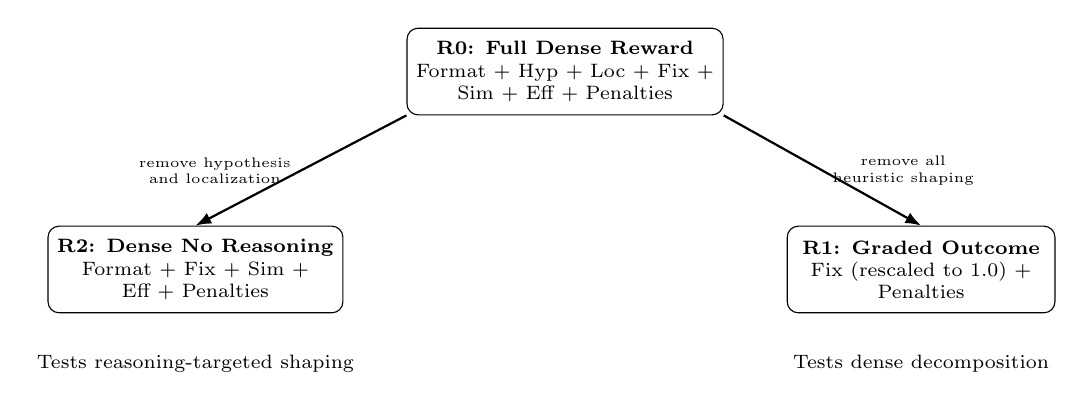
\begin{tikzpicture}[
    rewardbox/.style={
        draw,
        rounded corners,
        align=center,
        minimum width=3.4cm,
        minimum height=1.1cm,
        font=\scriptsize
    },
    arrow/.style={-{Latex[length=2mm]}, thick},
    label/.style={font=\tiny, align=center}
]

\node[rewardbox] (r0) {\textbf{R0: Full Dense Reward}\\Format + Hyp + Loc + Fix +\\Sim + Eff + Penalties};

\node[rewardbox, below left=1.4cm and 0.8cm of r0] (r2)
    {\textbf{R2: Dense No Reasoning}\\Format + Fix + Sim +\\Eff + Penalties};

\node[rewardbox, below right=1.4cm and 0.8cm of r0] (r1)
    {\textbf{R1: Graded Outcome}\\Fix (rescaled to 1.0) +\\Penalties};

\draw[arrow]
    (r0.south west) -- node[label, left]
    {remove hypothesis\\and localization}
    (r2.north);

\draw[arrow]
    (r0.south east) -- node[label, right]
    {remove all\\heuristic shaping}
    (r1.north);

\node[font=\scriptsize, below=0.4cm of r2]
    {Tests reasoning-targeted shaping};

\node[font=\scriptsize, below=0.4cm of r1]
    {Tests dense decomposition};

\end{tikzpicture}
\caption{Three reward configurations used in the controlled experiment, with component decompositions shown. R0--R1 provides a holistic comparison between composite heuristic shaping and monolithic outcome reward; R0--R2 cleanly isolates the targeted contribution of reasoning components (hypothesis and localization); R2--R1 compares remaining non-reasoning shaping terms against monolithic outcome reward.}
\label{fig:reward_flow}
\end{figure}

\begin{table}[h]
\centering
\small
\begin{tabular}{l c c c c l}
\toprule
\textbf{Component} & \textbf{R0} & \textbf{R1} & \textbf{R2} & \textbf{Maximum} & \textbf{Purpose} \\
\midrule
Format & \checkmark & --- & \checkmark & 0.10 & Five required response fields \\
Hypothesis & \checkmark & --- & --- & 0.20 & Grounded diagnosis \\
Localization & \checkmark & --- & --- & 0.15 & Function/line ID \\
Fix quality & \checkmark & \checkmark & \checkmark & 0.35 / 1.0 & Tests passed \\
Similarity & \checkmark & --- & \checkmark & 0.10 & Reference proximity \\
Efficiency & \checkmark & --- & \checkmark & 0.10 & Remaining-turn potential \\
Penalties & \checkmark & \checkmark & \checkmark & $-0.55$ & Invalid/regression \\
\bottomrule
\end{tabular}
\caption{Reward components across configurations. In R1, the Fix Quality ceiling is rescaled to 1.0 so that the total reward range is preserved.}
\label{tab:reward_components}
\end{table}

\subsection{Training}
We train Qwen2.5-Coder-3B-Instruct using GRPO with LoRA on the 90 training bugs for 500 optimizer steps. For the 24\,GB GPU profile used in the reported runs, LoRA uses rank 8 and $\alpha=16$, with batch size 2, gradient accumulation of 4, group size $G=2$, and a maximum completion length of 192 tokens for structured responses (Appendix~\ref{app:hyperparams}). By contrast, final greedy evaluations use 300 tokens for structured responses and 700 tokens for free-form responses. This completion budget disparity introduces an asymmetric truncation dynamic during training: when a completion is truncated before emitting the code block in \texttt{DETAIL}, R1 awards zero credit (or penalties) because no executable patch exists. However, R0 still awards up to $+0.45$ for prefix fields (\texttt{OBSERVATION}, \texttt{HYPOTHESIS}, and \texttt{LOCALIZATION}) that precede the code block. Consequently, R0 actively reinforced truncated non-solutions with positive reward during training, while R1 treated them as total failures. The reward intervention is therefore partially coupled to completion truncation: under the 192-token training budget, R0 can assign positive diagnostic credit to truncated responses whereas R1 cannot. We treat this as part of the tested reward configuration rather than an implementation artifact, but it limits interpretation of the result as a pure comparison of reward density. We use AdamW with learning rate $2\times10^{-5}$, cosine scheduling, 30 warmup steps in the first curriculum stage, and sampling temperature 0.7. The curriculum exposes tier 1 for steps 0--149, tiers 1--2 for steps 150--349, and all three tiers for steps 350--499. All three RL configurations use the same training configuration and differ only in reward definition. Full hyperparameters are provided in Appendix~\ref{app:hyperparams}.

\section{Experimental Design}

\subsection{Research Questions}
\begin{itemize}
\item \textbf{RQ1:} Does GRPO training improve held-out debugging over zero-shot baselines (both structured and free-form)?
\item \textbf{RQ2:} Does dense decomposition help? (R0 vs R1)
\item \textbf{RQ3:} Do reasoning-targeted components help? (R0 vs R2)
\item \textbf{RQ4:} Do trained policies transfer beyond the mutation-generated training distribution?
\end{itemize}

\subsection{Experimental Arms}
We conduct 3 independent training runs (seeds 42, 123, 456) for each of the three reward configurations (R0, R1, R2), producing 9 trained policies. We also evaluate the zero-shot base model in both structured format (B0) and unconstrained free-form format (B1).

\subsection{Evaluation}
Final evaluations use greedy decoding (temperature 0.0) on the 90 held-out bugs. We also conduct an exploratory external evaluation on 27 single-function adapted QuixBugs programs.

\subsection{Statistical Analysis}
Our primary analysis uses bug-level paired bootstrap intervals, averaging solve indicators across the three seeds before resampling bugs. For each bug $i$, we compute the seed-averaged solve indicator $\bar{s}_{i,\text{arm}} = \frac{1}{3}\sum_{k=1}^{3}s_{i,\text{arm},k}$. We bootstrap the $N=90$ bugs to compute the difference $\Delta = \frac{1}{N}\sum_i (\bar{s}_{i,\text{arm}_A}-\bar{s}_{i,\text{arm}_B})$. The primary bootstrap resamples evaluation bugs and therefore quantifies uncertainty over the evaluation-bug population conditional on the three observed training seeds. 

With $N=90$ paired bugs and 3 training seeds, a standard power analysis ($\alpha=0.05$, two-tailed, power $1-\beta=0.80$, under the observed paired-discordance rate across seeds) reveals that the minimum detectable effect (MDE) is approximately 16 percentage points for paired differences. The experiment is therefore powered primarily for large shifts in policy capability; subtle differences of a few percentage points cannot be detected. The 95\% bootstrap confidence interval for R0$-$R1 of [$-$8.5, $+$2.6] pp rules out a dense-reward advantage larger than 2.6 percentage points at the reported confidence level, while being consistent with small negative or near-zero differences. As a secondary sensitivity check, we apply exact McNemar tests~\cite{McNemar1947} to binary paired outcomes defined by majority vote across seeds (a bug is solved if $\ge 2/3$ seeds solve it), as well as per-seed paired evaluations (Appendix~\ref{app:stats}); across all comparisons, no contrast approaches statistical significance.

\paragraph{Deviations from Preregistration.}
The final study differs from the pre-registration specification in four material ways, all established prior to final matrix analysis:
\begin{enumerate}
\item \textbf{Model scale:} Primary training was executed at the 3B scale rather than 7B due to compute constraints (75 GPU-hours on 24\,GB RTX 4090 hardware).
\item \textbf{Omitted hypotheses:} Two secondary hypotheses from the pre-registration were dropped to concentrate full replication and power on the central reward decomposition question (H2):
\begin{itemize}
\item \textit{H1 (Structured Format):} The hypothesis that imposing an explicit Observation $\to$ Hypothesis $\to$ Action format constraint alone improves repair accuracy over unconstrained free-form generation.
\item \textit{H3 (Curriculum Anti-Collapse):} The hypothesis that a multi-tier progressive curriculum prevents early policy collapse on Tier 3 bugs compared to uniform training.
\end{itemize}
Neither dropped hypothesis is presented as confirmatory evidence.
\item \textbf{Difficulty gate calibration:} Difficulty gating calibration was performed with local Llama-3.1-8B-Instruct rather than external API calls.
\item \textbf{External transfer baseline:} The QuixBugs benchmark was evaluated without an untrained zero-shot B0 baseline, rendering its numbers strictly descriptive.
\end{enumerate}

\begin{table*}[t]
\centering
\small
\begin{tabular}{l c c l}
\toprule
\textbf{Comparison} & \textbf{Contrast} & \textbf{Prediction} & \textbf{Outcome} \\
\midrule
RQ2 & R0 vs R1 & Dense decomposition helps & Not supported \\
RQ3 & R0 vs R2 & Reasoning terms help & Not supported \\
Exploratory & R2 vs R1 & Non-reasoning shaping helps & Not supported \\
Transfer & External evaluation & Generalization beyond MBPP & Descriptive only (no B0 baseline) \\
\bottomrule
\end{tabular}
\caption{Summary of research questions, contrasts, predictions, and empirical outcomes.}
\label{tab:hypotheses}
\end{table*}

\section{Results}

\begin{table}[h]
\centering
\small
\begin{tabular}{l c c c}
\toprule
\textbf{Model} & \textbf{Train (In-Dist.)} & \textbf{Held-out (In-Dist.)} & \textbf{QuixBugs (External)} \\
\midrule
B0 (Structured Zero-Shot) & --- & 37.8\% & --- \\
B1 (Free-Form Zero-Shot)   & --- & 45.6\% & --- \\
E1 (R0 Full)              & 51.9\% $\pm$ 2.3 & 45.6\% $\pm$ 2.9 & 39.5\% $\pm$ 2.1 \\
E3 (R1 Graded Outcome)     & 54.4\% $\pm$ 3.3 & 48.5\% $\pm$ 6.5 & 43.2\% $\pm$ 5.7 \\
E4 (R2 No Reasoning)      & 51.5\% $\pm$ 3.6 & 48.5\% $\pm$ 3.9 & 44.4\% $\pm$ 3.7 \\
\bottomrule
\end{tabular}
\caption{Solve rate by split and RL configuration (Mean \% $\pm$ Std Dev across 3 seeds). Zero-shot baselines involve no training and were evaluated on the 90 held-out bugs. QuixBugs values are descriptive; no zero-shot baseline was evaluated on this external benchmark.}
\label{tab:results}
\end{table}

\subsection{Main Reward Comparison (Confirmatory)}
\textbf{Main result.} The full dense reward does not improve held-out debugging success relative to either ablated configuration. R0 solves 45.6\% of held-out bugs, versus 48.5\% for both R1 and R2. The point estimate therefore favors the simpler configurations, but the paired bootstrap interval for R0$-$R1, [$-$8.5, $+$2.6] percentage points, includes zero. This interval rules out a dense-reward advantage larger than 2.6 percentage points at the reported 95\% confidence level. We note that the value 45.6\% appears in three places in our data: (1) E1's held-out mean across three seeds (123/270 = 45.56\%), (2) the corrected free-form zero-shot baseline B1 (41/90 = 45.56\%), and (3) the recovered solve rate in the evaluation-harness analysis (§\ref{sec:harness}). All three refer to exact evaluations on the same 90 held-out bugs and reflect identical arithmetic proportions rather than a data-entry artifact.

\begin{table}[h]
\centering
\small
\begin{tabular}{l c c c}
\toprule
\textbf{Comparison} & \textbf{$\Delta$ Solve Rate} & \textbf{95\% Bootstrap CI} & \textbf{Holm-adjusted McNemar $p$} \\
\midrule
R0 $-$ R1 & $-$2.9 pp & [$-$8.5, $+$2.6] & 1.0000 \\
R0 $-$ R2 & $-$2.9 pp & [$-$8.5, $+$2.6] & 1.0000 \\
R2 $-$ R1 & 0.0 pp & [$-$5.6, $+$5.6] & 1.0000 \\
\bottomrule
\end{tabular}
\caption{Pairwise comparisons for held-out solve rates. All bootstrap intervals cross zero, and paired McNemar tests yield no statistically significant difference after Holm correction.}
\label{tab:pairwise}
\end{table}

All three pairwise comparisons yield no statistically detectable difference after Holm correction. Reasoning-targeted reward engineering, at this scale and task, bought no measurable performance.

\subsection{Reward Degeneracy and the G=2 Mechanism (Exploratory)}
The reward configurations produce substantially different GRPO training signals. Across logged training calls, the mean fraction of degenerate sampled groups (where all samples in a group receive rewards within the configured degeneracy tolerance $\Delta R < 10^{-6}$, resulting in zero relative advantage) was 16.2\% $\pm$ 2.2\% for R0 (individual seed means: 14.4\%, 15.6\%, 18.6\%), 61.9\% $\pm$ 4.2\% for R1 (seed means: 62.3\%, 65.9\%, 57.5\%), and 34.7\% $\pm$ 3.9\% for R2 (seed means: 38.3\%, 30.5\%, 35.3\%). The dense reward substantially reduces the frequency of groups in which sampled completions receive indistinguishable outcomes ($R0 - R1 = -45.7$ pp).

However, analyzing the advantage normalization mechanism under group size $G=2$ explains why this large reduction in degeneracy failed to improve held-out repair. For group size $G=2$, the standard deviation normalization removes the magnitude of the reward difference. With sampled rewards $R_1$ and $R_2$, the group mean is $\mu=(R_1+R_2)/2$ and the sample standard deviation used by our TRL implementation is $\sigma=|R_1-R_2|/\sqrt{2}$. Ignoring the small numerical stabilizer ($10^{-4}$), the normalized advantages are therefore:
\begin{equation}
A_1 = \frac{R_1-\mu}{\sigma} = \frac{(R_1-R_2)/2}{|R_1-R_2|/\sqrt{2}} = \frac{1}{\sqrt{2}}\operatorname{sign}(R_1-R_2), \qquad A_2 = -A_1
\end{equation}
Thus, the key structural property is not the exact numerical magnitude of the advantage ($\pm 1/\sqrt{2}$), but that its magnitude is completely independent of the size of the reward difference. A reward gap of $0.001$ and a gap of $0.5$ produce the exact same absolute advantage magnitude. Under $G=2$, dense shaping therefore acts primarily as a tie-breaker whenever it alters the relative ordering of the two completions.

In R1 (outcome-only), when both sampled completions fail all test cases, $R_1 = R_2 = 0$, producing a degenerate group with zero advantage and no parameter update. In R0 (dense reward), even when both completions fail all tests, heuristic shaping components (such as minor variations in hypothesis phrasing, keyword presence, or reference token similarity) routinely produce unequal scalar rewards ($R_1 \ne R_2$). Under $G=2$, this assigns the two completions equal-magnitude positive and negative advantages of approximately $\pm 1/\sqrt{2}$. In groups where both candidates fail all tests, this can convert an otherwise degenerate outcome tie into a same-magnitude heuristic tie-breaker, assigning equal-magnitude normalized advantages based on heuristic scoring rather than functional correctness.

\begin{figure*}[t]
\centering
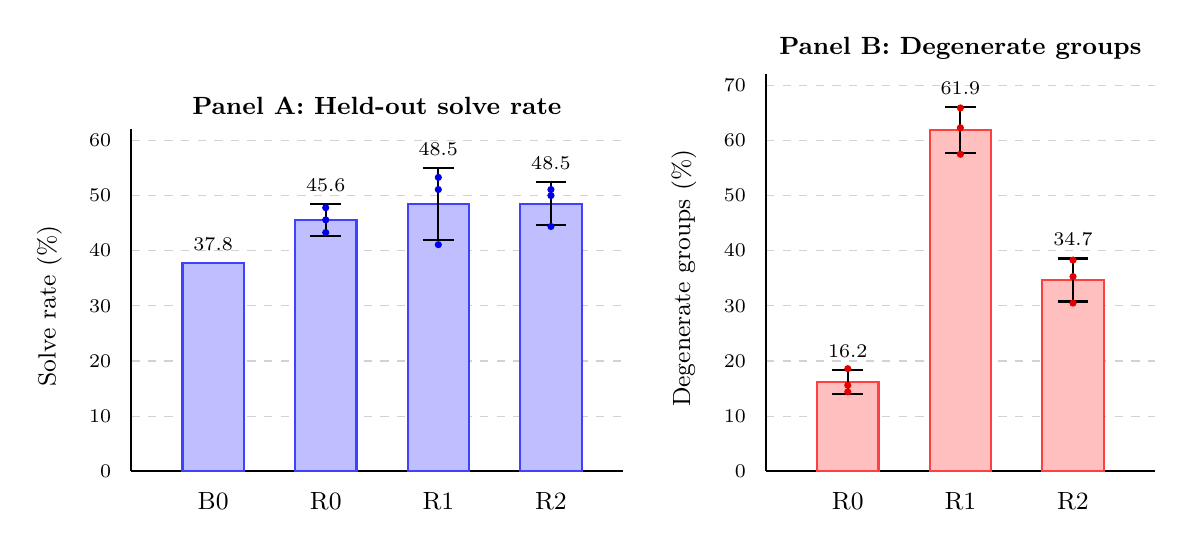
\begin{tikzpicture}[x=1.3cm, y=0.07cm]
    % Left Panel: Solve rate
    \begin{scope}[shift={(0,0)}]
        \foreach \y in {0, 10, 20, 30, 40, 50, 60} {
            \draw[dashed, gray!35] (0, \y) -- (4.8, \y);
            \node[anchor=east, font=\scriptsize] at (-0.1, \y) {\y};
        }
        \draw[thick] (0,0) -- (4.8,0);
        \draw[thick] (0,0) -- (0,62);
        \node[rotate=90, font=\small, anchor=center] at (-0.8, 30) {Solve rate (\%)};
        
        % B0
        \draw[fill=blue!25, draw=blue!75, thick] (0.5,0) rectangle (1.1, 37.8);
        \node[font=\scriptsize, anchor=south] at (0.8, 38.3) {37.8};
        \node[font=\small, anchor=north] at (0.8, -2) {B0};
        
        % R0
        \draw[fill=blue!25, draw=blue!75, thick] (1.6,0) rectangle (2.2, 45.6);
        \draw[thick] (1.9, 45.6 - 2.9) -- (1.9, 45.6 + 2.9);
        \draw[thick] (1.75, 45.6 - 2.9) -- (2.05, 45.6 - 2.9);
        \draw[thick] (1.75, 45.6 + 2.9) -- (2.05, 45.6 + 2.9);
        \fill[blue!90!black] (1.9, 43.3) circle (1.3pt);
        \fill[blue!90!black] (1.9, 45.6) circle (1.3pt);
        \fill[blue!90!black] (1.9, 47.8) circle (1.3pt);
        \node[font=\scriptsize, anchor=south] at (1.9, 49.0) {45.6};
        \node[font=\small, anchor=north] at (1.9, -2) {R0};
        
        % R1
        \draw[fill=blue!25, draw=blue!75, thick] (2.7,0) rectangle (3.3, 48.5);
        \draw[thick] (3.0, 48.5 - 6.5) -- (3.0, 48.5 + 6.5);
        \draw[thick] (2.85, 48.5 - 6.5) -- (3.15, 48.5 - 6.5);
        \draw[thick] (2.85, 48.5 + 6.5) -- (3.15, 48.5 + 6.5);
        \fill[blue!90!black] (3.0, 41.1) circle (1.3pt);
        \fill[blue!90!black] (3.0, 51.1) circle (1.3pt);
        \fill[blue!90!black] (3.0, 53.3) circle (1.3pt);
        \node[font=\scriptsize, anchor=south] at (3.0, 55.5) {48.5};
        \node[font=\small, anchor=north] at (3.0, -2) {R1};
        
        % R2
        \draw[fill=blue!25, draw=blue!75, thick] (3.8,0) rectangle (4.4, 48.5);
        \draw[thick] (4.1, 48.5 - 3.9) -- (4.1, 48.5 + 3.9);
        \draw[thick] (3.95, 48.5 - 3.9) -- (4.25, 48.5 - 3.9);
        \draw[thick] (3.95, 48.5 + 3.9) -- (4.25, 48.5 + 3.9);
        \fill[blue!90!black] (4.1, 44.4) circle (1.3pt);
        \fill[blue!90!black] (4.1, 50.0) circle (1.3pt);
        \fill[blue!90!black] (4.1, 51.1) circle (1.3pt);
        \node[font=\scriptsize, anchor=south] at (4.1, 52.9) {48.5};
        \node[font=\small, anchor=north] at (4.1, -2) {R2};
        
        \node[font=\small\bfseries, anchor=south] at (2.4, 63) {Panel A: Held-out solve rate};
    \end{scope}

    % Right Panel: Degenerate groups
    \begin{scope}[shift={(6.2,0)}]
        \foreach \y in {0, 10, 20, 30, 40, 50, 60, 70} {
            \draw[dashed, gray!35] (0, \y) -- (3.8, \y);
            \node[anchor=east, font=\scriptsize] at (-0.1, \y) {\y};
        }
        \draw[thick] (0,0) -- (3.8,0);
        \draw[thick] (0,0) -- (0,72);
        \node[rotate=90, font=\small, anchor=center] at (-0.8, 35) {Degenerate groups (\%)};
        
        % R0: 16.2 +- 2.2
        \draw[fill=red!25, draw=red!75, thick] (0.5,0) rectangle (1.1, 16.2);
        \draw[thick] (0.8, 16.2 - 2.2) -- (0.8, 16.2 + 2.2);
        \draw[thick] (0.65, 16.2 - 2.2) -- (0.95, 16.2 - 2.2);
        \draw[thick] (0.65, 16.2 + 2.2) -- (0.95, 16.2 + 2.2);
        \fill[red!90!black] (0.8, 14.4) circle (1.3pt);
        \fill[red!90!black] (0.8, 15.6) circle (1.3pt);
        \fill[red!90!black] (0.8, 18.6) circle (1.3pt);
        \node[font=\scriptsize, anchor=south] at (0.8, 18.9) {16.2};
        \node[font=\small, anchor=north] at (0.8, -2) {R0};
        
        % R1: 61.9 +- 4.2
        \draw[fill=red!25, draw=red!75, thick] (1.6,0) rectangle (2.2, 61.9);
        \draw[thick] (1.9, 61.9 - 4.2) -- (1.9, 61.9 + 4.2);
        \draw[thick] (1.75, 61.9 - 4.2) -- (2.05, 61.9 - 4.2);
        \draw[thick] (1.75, 61.9 + 4.2) -- (2.05, 61.9 + 4.2);
        \fill[red!90!black] (1.9, 57.5) circle (1.3pt);
        \fill[red!90!black] (1.9, 62.3) circle (1.3pt);
        \fill[red!90!black] (1.9, 65.9) circle (1.3pt);
        \node[font=\scriptsize, anchor=south] at (1.9, 66.6) {61.9};
        \node[font=\small, anchor=north] at (1.9, -2) {R1};
        
        % R2: 34.7 +- 3.9
        \draw[fill=red!25, draw=red!75, thick] (2.7,0) rectangle (3.3, 34.7);
        \draw[thick] (3.0, 34.7 - 3.9) -- (3.0, 34.7 + 3.9);
        \draw[thick] (2.85, 34.7 - 3.9) -- (3.15, 34.7 - 3.9);
        \draw[thick] (2.85, 34.7 + 3.9) -- (3.15, 34.7 + 3.9);
        \fill[red!90!black] (3.0, 30.5) circle (1.3pt);
        \fill[red!90!black] (3.0, 35.3) circle (1.3pt);
        \fill[red!90!black] (3.0, 38.3) circle (1.3pt);
        \node[font=\scriptsize, anchor=south] at (3.0, 39.1) {34.7};
        \node[font=\small, anchor=north] at (3.0, -2) {R2};
        
        \node[font=\small\bfseries, anchor=south] at (1.9, 73) {Panel B: Degenerate groups};
    \end{scope}
\end{tikzpicture}
\caption{Held-out solve rate and GRPO reward degeneracy. Bars show mean values across three seeds; error bars indicate standard deviation across seeds, with filled dots displaying individual seed runs. Degeneracy values show the mean fraction of degenerate sampled groups across the three seeds, with error bars showing the standard deviation across seed-level means. The dense reward substantially changes the training signal while producing no detectable improvement in held-out solve rate.}
\label{fig:main_results}
\end{figure*}

However, this difference does not translate into higher held-out solve rate. R1 also exhibits greater across-seed variance (std dev $\pm 6.5$ vs $\pm 2.9$), consistent with---but insufficient to establish---the hypothesis that increased reward degeneracy produces noisier, less stable optimization. Three seeds are insufficient for a formal variance comparison. This establishes an association between reward configuration and group degeneracy, not a causal relationship between degeneracy and final performance.

\subsection{Zero-Shot Baselines and Format Analysis (Exploratory)}
Comparing the nine RL runs against zero-shot baselines illuminates the source of the observed performance change. Against the structured zero-shot baseline B0 (37.8\%), the pooled RL runs (mean 47.5\%) show an apparent gain of +9.7 percentage points (bootstrap 95\% CI [1.0, 18.5]). However, the free-form zero-shot baseline with adequate generation budget (B1 corrected) achieves 45.6\% on the exact same 90 held-out bugs. Relative to this unconstrained zero-shot baseline, the best RL configuration (48.5\%) provides an increase of only +2.9 percentage points, and the pooled RL gain is only +1.9 percentage points—small relative to the across-seed variation observed among the RL arms (e.g., standard deviation of $\pm 6.5$ pp in R1).

This comparison reveals that imposing the rigid five-field structured format initially penalized the pre-trained base model, dropping its solve rate from 45.6\% to 37.8\% (a 7.8 pp penalty). This pattern is consistent with GRPO primarily recovering performance lost to the structured-response constraint rather than producing a large increase in underlying repair capability over unconstrained generation. The train--held-out gap across the nine RL runs is approximately 6 percentage points (52.6\% vs 47.5\%), showing modest in-distribution overfitting.

\subsection{External-Source Transfer (Exploratory)}
We evaluate the trained policies on a 27-program external set adapted from QuixBugs. E1, E3, and E4 achieve 39.5\% $\pm$ 2.1\%, 43.2\% $\pm$ 5.7\%, and 44.4\% $\pm$ 3.7\%, respectively. These numbers serve as a descriptive out-of-distribution sanity check that the policies maintain non-trivial repair behavior outside the synthetic MBPP mutation distribution. However, because we did not evaluate an untrained zero-shot B0 baseline on this external set, these measurements cannot distinguish whether this performance reflects transfer acquired through RL training or simply the base model's pre-existing code generation competence. We therefore report them strictly as descriptive out-of-distribution observations rather than evidence of an RL transfer advantage.

\subsection{Evaluation-Harness Case Study (Exploratory)}
\label{sec:harness}
Our initial zero-shot baseline experiments uncovered an evaluation-harness artifact that illustrates the sensitivity of code-RL benchmarking to generation constraints.

\begin{table}[h]
\centering
\small
\begin{tabular}{l c c c}
\toprule
\textbf{Configuration} & \textbf{Max tokens} & \textbf{Extraction failure} & \textbf{Solve rate} \\
\midrule
B1 initial (free-form) & 300 & 86.7\% & 1.1\% \\
B1 corrected (free-form) & 700 & < 5.0\% & 45.6\% \\
B0 structured & 300 & < 5.0\% & 37.8\% \\
\bottomrule
\end{tabular}
\caption{Impact of generation budget on evaluation fidelity. Free-form responses require extended budgets to complete explanatory prose before emitting code blocks; structured responses emit code within 300 tokens (training used 192 tokens).}
\label{tab:truncation}
\end{table}

When evaluated under a restrictive 300-token budget, the free-form zero-shot baseline suffered an 86.7\% extraction failure rate because verbose explanatory prose was truncated before the code block was generated, suppressing solve rate to 1.1\%. Expanding the budget to 700 tokens restored solve rate to 45.6\%. This 44.5 percentage point swing highlights how prompt format and budget parameters can induce substantial artifacts that dwarf the reward shaping effects under study.

\section{Discussion}
The seven-component reward introduces hundreds of lines of heuristic scoring logic and several independently chosen design thresholds, each introducing an additional opportunity for reward misspecification or exploitation. Despite this engineering effort, the simpler graded outcome reward was sufficient to achieve comparable held-out performance. 

\subsection{Why Did Dense Reward Fail to Improve Solve Rate?}
Three complementary mechanisms explain this result:
\begin{enumerate}
\item \textbf{Equal-magnitude advantages under $G=2$:} As derived in Equation 4, sample standard deviation normalization at $G=2$ eliminates the magnitude of reward differences ($|A| = 1/\sqrt{2}$). In groups where both completions fail all tests, R1 yields zero relative advantage, whereas R0 assigns equal-magnitude normalized advantages driven by heuristic tie-breakers (format compliance, keyword matching, reference similarity). R0 therefore assigned same-magnitude advantage weighting to heuristic distinctions that were not directly tied to functional correctness.
\item \textbf{Asymmetric truncation during training:} With training completions capped at 192 tokens on 24\,GB hardware, cut-off completions that failed to emit code received zero reward under R1, but collected up to $+0.45$ under R0 for prefix diagnostic fields. The reward intervention is therefore partially coupled to completion truncation: under the 192-token training budget, R0 can assign positive diagnostic credit to truncated responses whereas R1 cannot. We treat this as part of the tested reward configuration rather than an implementation artifact, but it limits interpretation of the result as a pure comparison of reward density.
\item \textbf{Reward-agnostic elicitation in pre-trained models:} Consistent with the findings of Shao et al.~\cite{Shao2025Spurious}, RLVR on open reasoning models often functions as format elicitation and latent knowledge activation rather than reward-guided search. This is reinforced by our baseline comparison: RL gained only +1.9 pp over the model's natural free-form baseline (45.6\%), consistent with the interpretation that training primarily elicited schema compliance rather than discovering fundamentally new repair heuristics.
\end{enumerate}

\section{Limitations and Scope}
\begin{itemize}
\item \textbf{Model scale:} Only Qwen2.5-Coder-3B.
\item \textbf{Algorithm:} Only GRPO.
\item \textbf{Group size $G=2$:} Sample standard deviation normalization at $G=2$ eliminates reward magnitude, scaling all non-zero reward differences to the same absolute advantage ($\pm 1/\sqrt{2}$). This prevents dense shaping from providing proportional advantage scaling and reduces its role to a tie-breaker.
\item \textbf{Completion budget disparity and truncation coupling:} Training used a 192-token completion cap, asymmetrically rewarding truncated non-solutions under R0 (+0.45 for prefix fields) while awarding zero under R1. Evaluation used 300 tokens for structured and 700 for free-form.
\item \textbf{Task structure:} Single-function, single-turn. Multi-step debugging may present a different regime in which intermediate rewards could be substantially more valuable.
\item \textbf{Bug distribution:} Mutation-generated MBPP bugs.
\item \textbf{Transfer set:} Only 27 adapted QuixBugs programs evaluated without a zero-shot baseline, rendering external numbers descriptive.
\item \textbf{Seeds:} Only 3 per arm, limiting robust variance estimates.
\item \textbf{Statistical power:} Large paired effects ($\ge 16$ pp MDE) are detectable; small effects of a few percentage points are not.
\item \textbf{Reward design:} Our ``dense reward'' is one particular handcrafted design, not all dense rewards. This study does not establish that dense rewards do not work, only that this specific decomposition did not improve this task.
\end{itemize}

\paragraph{What this study does NOT establish.}
Dense reward shaping never helps; Outcome reward is universally sufficient; Reasoning rewards are useless; GRPO is superior to other RL algorithms; 3B debugging results transfer to frontier models; Single-turn debugging results apply to agentic repository-level debugging; QuixBugs establishes robust generalization.

\section{Conclusion}
The most informative result is not simply that the dense reward failed to improve solve rate. It is that it changed the optimization signal substantially: R0 produced far fewer degenerate GRPO groups than R1, yet this advantage did not translate into higher held-out performance. Under group size $G=2$, advantage standardization completely eliminates reward magnitude, converting heuristic differences on identical test failures into full-scale normalized advantages. The result separates two quantities that are often implicitly conflated: within-group reward discrimination and the usefulness of the resulting advantage signal. Furthermore, generation budget mismatches can induce spurious performance swings that dwarf subtle reward differences, demonstrating that artifact validation is integral to empirical RL evaluation.

\textbf{Practical takeaway.} If a code-RL system already obtains meaningful executable feedback from a moderately capable base model, first establish that the outcome reward is insufficient before introducing additional heuristic reasoning rewards. Such shaping may reduce reward degeneracy, but our results show that this optimization benefit need not translate into better final repair accuracy.

\bibliographystyle{plain}
\begin{thebibliography}{12}
\bibitem{Austin2021} Austin, J., Odena, A., Nye, M., et al. (2021). Program Synthesis with Large Language Models. arXiv:2108.07732.
\bibitem{Guo2025} Guo, D., et al. (2025). DeepSeek-R1: Incentivizing Reasoning Capability in LLMs via Reinforcement Learning. arXiv:2501.12948.
\bibitem{Lightman2023} Lightman, H., et al. (2023). Let's Verify Step by Step. ICLR 2024. arXiv:2305.20050.
\bibitem{Lin2017} Lin, D., et al. (2017). QuixBugs: A Multi-Lingual Program Repair Benchmark Set Based on the Quixey Challenge. SPLASH Companion 2017.
\bibitem{McNemar1947} McNemar, Q. (1947). Note on the sampling error of the difference between correlated proportions or percentages. Psychometrika, 12(2), 153--157.
\bibitem{Ng1999} Ng, A. Y., Harada, D., \& Russell, S. (1999). Policy invariance under reward transformations: Theory and application to reward shaping. ICML 1999.
\bibitem{Shao2024} Shao, Z., et al. (2024). DeepSeekMath: Pushing the Limits of Mathematical Reasoning in Open Language Models. arXiv:2402.03300.
\bibitem{Shao2025Spurious} Shao, Y., et al. (2025). Spurious Rewards: Rethinking Training Signals in RLVR. arXiv:2506.10947.
\bibitem{Tam2024} Tam, Z. R., et al. (2024). Let Me Speak Freely? Long-Form Thinking and Evaluation Artifacts. EMNLP 2024. arXiv:2408.02442.
\bibitem{Tian2024} Tian, R., et al. (2024). DebugBench: Evaluating Large Language Models for Program Debugging. ACL 2024. arXiv:2401.04621.
\bibitem{Uesato2022} Uesato, J., et al. (2022). Solving Math Word Problems with Process- and Outcome-based Feedback. arXiv:2211.14275.
\bibitem{Zheng2025Contamination} Zheng, C., et al. (2025). Investigating Data Contamination and Reasoning in Open-Weight Code Models. arXiv:2507.10532.
\end{thebibliography}

\clearpage
\appendix

\section{Training Hyperparameters}
\label{app:hyperparams}

Table~\ref{tab:hyperparams} reports the training hyperparameters for the reported 24\,GB GPU runs. All reward component ceilings and penalty magnitudes were fixed in the pre-registered environment specification before the reported training runs; they were not tuned against held-out solve rates. The curriculum schedule is given in Table~\ref{tab:curriculum}.

\begin{table}[h]
\centering
\small
\begin{tabular}{ll}
\toprule
\textbf{Parameter} & \textbf{Value} \\
\midrule
Base model & Qwen/Qwen2.5-Coder-3B-Instruct \\
RL algorithm & GRPO \\
LoRA rank & 8 \\
LoRA $\alpha$ & 16 \\
LoRA dropout & 0.0 \\
LoRA target modules & q\_proj, k\_proj, v\_proj, o\_proj, gate\_proj, up\_proj, down\_proj \\
Optimizer & AdamW \\
Learning rate & $2\times10^{-5}$ \\
Scheduler & cosine \\
Warmup & 30 steps (stage 1 only) \\
Total optimizer steps & 500 \\
Group size $G$ & 2 \\
Per-device batch size & 2 \\
Gradient accumulation steps & 4 \\
Structured completion budget (training) & 192 tokens \\
Evaluation completion budget (structured / free-form) & 300 / 700 tokens \\
Sampling temperature & 0.7 \\
Reward workers & 1 \\
Seeds & 42, 123, 456 \\
\bottomrule
\end{tabular}
\caption{Training hyperparameters for the reported 24\,GB GPU runs.}
\label{tab:hyperparams}
\end{table}

\begin{table}[h]
\centering
\small
\begin{tabular}{c c l}
\toprule
\textbf{Curriculum Stage} & \textbf{Training Steps} & \textbf{Active Tiers} \\
\midrule
Stage 0 & 0--149 & Tier 1 (Easy) \\
Stage 1 & 150--349 & Tiers 1--2 (Easy, Medium) \\
Stage 2 & 350--499 & Tiers 1--3 (Easy, Medium, Hard) \\
\bottomrule
\end{tabular}
\caption{Curriculum schedule used in all three RL configurations.}
\label{tab:curriculum}
\end{table}

\paragraph{Curriculum-stage optimization.}
Training is implemented as three sequential GRPO trainers, one per curriculum stage. The LoRA adapter is carried across stages, while each stage initializes a fresh optimizer and scheduler. Only the first stage uses the 30-step warmup; later stages restart the cosine schedule at the configured learning rate without warmup. This implementation detail is shared across R0, R1, and R2.

\section{Statistical Analysis Details}
\label{app:stats}

\subsection{Primary Paired Bootstrap}
For each bug $i \in \{1, \dots, 90\}$, the solve indicator is averaged across the three seeds:
\begin{equation}
\bar{s}_{i,\text{arm}} = \frac{1}{3}\sum_{k=1}^{3} s_{i,\text{arm},k}
\end{equation}
The analysis script also verifies that all nine RL result files contain the same 90 held-out bug identifiers and that the train and held-out bug IDs are disjoint before computing intervals. We resample the $N=90$ bugs with replacement 10,000 times (fixed RNG seed 204) to generate the empirical distribution of paired differences $\Delta = \frac{1}{N}\sum_{i=1}^{N}(\bar{s}_{i,\text{arm}_A} - \bar{s}_{i,\text{arm}_B})$. Percentile endpoints at 2.5\% and 97.5\% define the 95\% confidence intervals.

\subsection{Secondary McNemar Sensitivity Analysis}
To evaluate sensitivity, we apply exact paired binomial McNemar tests to discordant pairs. For the majority-vote analysis, all three Holm-adjusted $p$-values are 1.0000. The per-seed sensitivity analyses likewise yield no statistically significant contrast after Holm correction; the smallest adjusted $p$-value is 0.2780.

\begin{table}[h]
\centering
\small
\begin{tabular}{l c c c c c c}
\toprule
\textbf{Comparison} & \textbf{Arm A Solved} & \textbf{Arm B Solved} & \textbf{A-only} & \textbf{B-only} & \textbf{Raw $p$} & \textbf{Holm-adj $p$} \\
\midrule
E1 vs E3 & 42/90 (46.7\%) & 44/90 (48.9\%) & 8 & 10 & 0.8145 & 1.0000 \\
E1 vs E4 & 42/90 (46.7\%) & 44/90 (48.9\%) & 6 & 8 & 0.7905 & 1.0000 \\
E3 vs E4 & 44/90 (48.9\%) & 44/90 (48.9\%) & 7 & 7 & 1.0000 & 1.0000 \\
\bottomrule
\end{tabular}
\caption{Majority-vote McNemar tests on held-out bugs (a bug is considered solved if solved by $\ge 2/3$ seeds).}
\label{tab:mcnemar_majority}
\end{table}

\begin{table}[h]
\centering
\small
\begin{tabular}{l c c c c c c}
\toprule
\textbf{Comparison} & \textbf{Seed} & \textbf{A-only} & \textbf{B-only} & \textbf{Discordant} & \textbf{Raw $p$} & \textbf{Holm-adj $p$} \\
\midrule
E1 vs E3 & s42  & 13 & 7  & 20 & 0.2632 & 1.0000 \\
E1 vs E3 & s123 & 12 & 16 & 28 & 0.5716 & 1.0000 \\
E1 vs E3 & s456 & 5  & 15 & 20 & 0.0414 & 0.3311 \\
E1 vs E4 & s42  & 9  & 13 & 22 & 0.5235 & 1.0000 \\
E1 vs E4 & s123 & 7  & 9  & 16 & 0.8036 & 1.0000 \\
E1 vs E4 & s456 & 9  & 11 & 20 & 0.8238 & 1.0000 \\
E3 vs E4 & s42  & 4  & 14 & 18 & 0.0309 & 0.2780 \\
E3 vs E4 & s123 & 12 & 10 & 22 & 0.8318 & 1.0000 \\
E3 vs E4 & s456 & 12 & 4  & 16 & 0.0768 & 0.5377 \\
\bottomrule
\end{tabular}
\caption{Per-seed exact McNemar tests across the 9 individual runs.}
\label{tab:mcnemar_perseed}
\end{table}

\section{External Transfer Set (QuixBugs)}
\label{app:quixbugs}

The external transfer benchmark consists of 27 single-function Python programs adapted from the QuixBugs dataset \cite{Lin2017}. Out of 40 original QuixBugs programs, 13 were excluded because their argument or return shapes required custom pointer/graph structures not representable in JSON (e.g., linked list or graph nodes) or used generator yields without list wrapping. 

The 27 validated candidate programs are listed in Table~\ref{tab:quixbugs_list}. All programs were verified with our sandbox validator: the reference code passes 100\% of test cases, and the buggy code fails at least one case. Because no zero-shot B0 baseline was executed on this external set, performance is reported descriptively.

\begin{table}[h]
\centering
\footnotesize
\begin{tabular}{lll}
\toprule
\multicolumn{3}{c}{\textbf{QuixBugs Program Identifiers (27 Programs)}} \\
\midrule
\texttt{quixbugs\_bitcount} & \texttt{quixbugs\_bucketsort} & \texttt{quixbugs\_find\_first\_in\_sorted} \\
\texttt{quixbugs\_find\_in\_sorted} & \texttt{quixbugs\_gcd} & \texttt{quixbugs\_get\_factors} \\
\texttt{quixbugs\_is\_valid\_parenthesization} & \texttt{quixbugs\_knapsack} & \texttt{quixbugs\_kth} \\
\texttt{quixbugs\_lcs\_length} & \texttt{quixbugs\_levenshtein} & \texttt{quixbugs\_lis} \\
\texttt{quixbugs\_longest\_common\_subsequence} & \texttt{quixbugs\_max\_sublist\_sum} & \texttt{quixbugs\_mergesort} \\
\texttt{quixbugs\_next\_palindrome} & \texttt{quixbugs\_next\_permutation} & \texttt{quixbugs\_pascal} \\
\texttt{quixbugs\_possible\_change} & \texttt{quixbugs\_powerset} & \texttt{quixbugs\_quicksort} \\
\texttt{quixbugs\_rpn\_eval} & \texttt{quixbugs\_shunting\_yard} & \texttt{quixbugs\_sieve} \\
\texttt{quixbugs\_subsequences} & \texttt{quixbugs\_to\_base} & \texttt{quixbugs\_wrap} \\
\bottomrule
\end{tabular}
\caption{Identifiers of the 27 adapted QuixBugs programs used for external transfer evaluation.}
\label{tab:quixbugs_list}
\end{table}

\section{Artifact Reproducibility}
\label{app:artifact}

Table~\ref{tab:artifacts} lists the primary repository locations of all datasets, rewards, training pipelines, and results.

\begin{table}[h]
\centering
\small
\begin{tabular}{ll}
\toprule
\textbf{Artifact} & \textbf{Location} \\
\midrule
Dataset & \texttt{src/agentdebugger/dataset/bugs/} \\
Fixed train/held-out split & \texttt{src/agentdebugger/dataset/bugs/} \\
QuixBugs external set & \texttt{data/quixbugs/} \\
Reward implementation & \texttt{src/agentdebugger/rewards/} \\
Curriculum environment & \texttt{src/agentdebugger/envs/curriculum\_env.py} \\
Training implementation & \texttt{src/agentdebugger/training/grpo.py} \\
Per-run evaluation results & \texttt{results/primary/E*\_s*.json} \\
Diagnostic evaluations & \texttt{results/diagnostics/} \\
Statistical analysis scripts & \texttt{analysis/bootstrap.py}, \texttt{analysis/analyze\_wandb.py} \\
Dataset construction & \texttt{scripts/build\_dataset.py} \\
QuixBugs adaptation script & \texttt{scripts/build\_quixbugs.py} \\
\bottomrule
\end{tabular}
\caption{Locations of the primary experimental artifacts in the released repository.}
\label{tab:artifacts}
\end{table}

\section{Evaluation-Harness Failure Analysis}
\label{app:harness}

During preliminary zero-shot evaluation, free-form completions were evaluated with a generation limit of 300 tokens. Free-form responses typically emitted thorough analytical prose before outputting the code fix block. Consequently, completions routinely exhausted the 300-token limit before reaching the closing code fence, resulting in an 86.7\% extraction failure rate and an apparent solve rate of only 1.1\%. 

Increasing the token limit to 700 tokens allowed models to complete both their analytical reasoning and the final code block, dropping extraction failures below 5\% and restoring the solve rate to 45.6\% (a 44.5 percentage point increase). This finding emphasizes that benchmark evaluation harnesses can introduce massive confounding effects that completely overshadow the algorithmic interventions under study.

\end{document}
